\section{The WSN construction}
\begin{frame}{The WSN construction}
    \centering
    Published by \href{https://doi.org/10.1007/978-3-662-48800-3_18}{Tessaro at AsiaCrypt 2015} [\texttt{\href{https://ia.cr/2015/868}{ia.cr/2015/868}}].
    \begin{columns}
        \begin{column}{0.49\textwidth}
            \begin{block}{Overview\vpPp}
                \centering
                \vspace*{13pt}
                \begin{tikzpicture}[scale=1]
                    \tikzstyle{every node}=[transform shape];

                    \node (mux) [trapezium, trapezium angle=-60, rounded corners=2pt, minimum width=20mm, draw, thick] {$0/1$};

                    \node (f) [left=7mm of mux,rectangle, rounded corners=2pt, minimum width=10mm, minimum height=15mm, draw, thick] {$f_i$};
                    \node (f-w) [left=-5pt of f.north,yshift=6.75mm] {\vphantom{$k$}$w_i$};
                    \node (f-k) [right=0.0mm of f.north,yshift=-1.25mm] {};
                    \node (k) [right=5.5mm of f.north,yshift=6.75mm] {$k_i$};
                    \draw[thick] (k) -- +(0,-3.5mm);

                    \node (xor) [below=5mm of mux.south, XOR] {};

                    \node (input) [left=30mm of xor] {$x_i$};
                    \node (output) [right=10mm of xor] {$x_{i+1}$};

                    \node (mux-k) [left=2.5mm of mux.north,yshift=-1.25mm] {};

                    %f input
                    \draw[thick, -latex] (input.east)+(2.5mm,0) -| (f.south);
                    \draw[thick, -latex] (f-w) -- +(0,-6.75mm);
                    \draw[thick, -latex] (k)+(0,-3.5mm) -| (f-k);
                    \draw[thick, -latex] (k)+(0,-3.5mm) -| (mux-k);

                    %mux input
                    \node (mux-zero) [right=2.5mm of mux.north,yshift=2.5mm+7mm] {0};
                    \draw[thick, -latex] (mux-zero.south) -- +(0,-7.125mm);

                    % mux control
                    \draw[thick, -latex] (f.east) -- (mux.west);

                    % xor input
                    \draw[thick, -latex] (input.east) -- (xor.west);
                    \draw[thick, -latex] (mux.south) -- (xor.north);

                    \draw[thick, -latex] (xor.east) -- (output.west);
                \end{tikzpicture}
                \vspace*{13pt}
            \end{block}
        \end{column}
        \begin{column}{0.49\textwidth}
            \begin{block}{Whitened Swap-Or-Not round function}
                \vspace*{-10pt}
                \begin{equation*}
                    x_i \mapsto x_i + f_{b(i)}(w_i + \max \set{x_i, x_i + k_i}) \cdot k_i
                \end{equation*}
            \end{block}

            \begin{block}{Security Proposition (informal)}
                The WSN construction with $\mathcal{O}(n)$ rounds is
                \begin{equation*}
                    (2^{n-\mathcal{O}(\log n)}, 2^{n-\mathcal{O}(1)})\text{-secure}.
                \end{equation*}
            \end{block}
        \end{column}
    \end{columns}
    \begingroup
        \vspace{10pt}
        \footnotesize
        $(p, q)$-secure: Attackers querying the encryption at most $p$ and the underlying $f_i$'s $q$ times have only negl.\ advantage.
    \endgroup
    \blfootnote{}
\end{frame}

\begin{frame}{An Implementation}
    \visible<2->{%
    \begin{minipage}{0.40\textwidth}
        \centering
        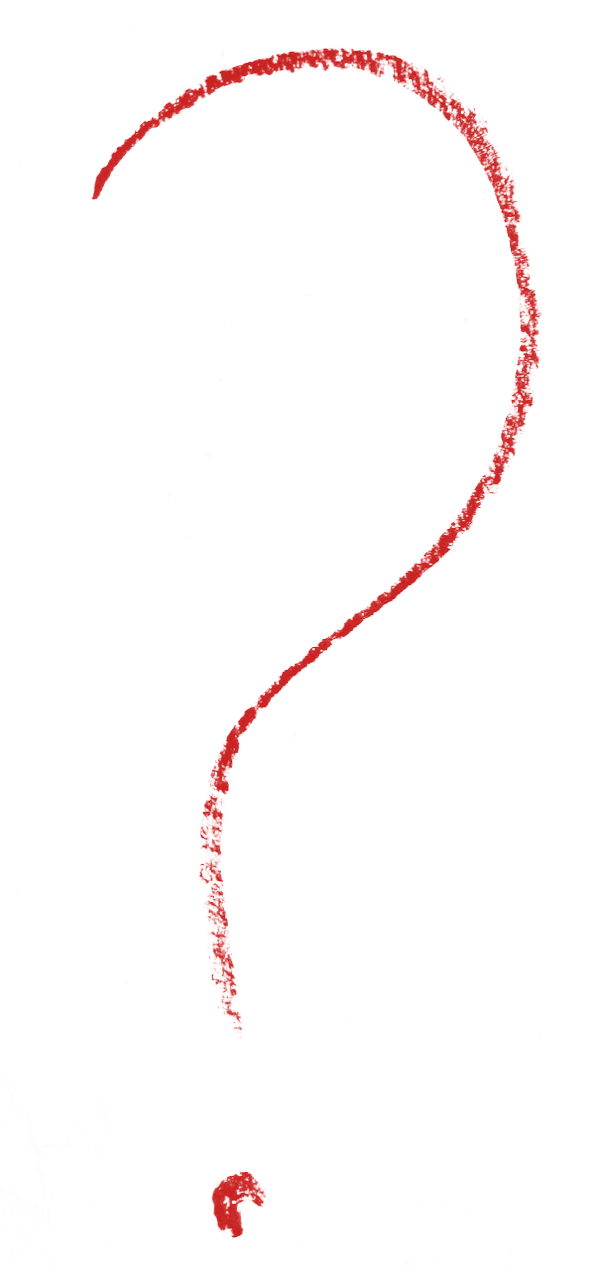
\includegraphics[height=0.6\textheight]{data/flickr/questionmark-alertred}
    \end{minipage}
    \hfill
    \begin{minipage}{0.56\textwidth}
        \centering
        \begin{block}{Construction}
            \begin{itemize}
                \item $f(x) \coloneqq\ $?
                \item Key schedule?
                \item $\mathcal{O}(n)$ rounds?
            \end{itemize}
        \end{block}
        \vspace{5pt}
        Theoretical vs.\ practical constructions
    \end{minipage}
    }
\end{frame}

\section{Generic Analysis}
\begin{frame}{Generic Analysis}{On the number of rounds}
    \centering
    \only<1>{%
    \begin{forest}
        %for tree={grow=east},
        [{$\makebox[6pt][c]{$p$}$}, name=root
            [{$\makebox[6pt][c]{$p$}$}
                [{$\makebox[6pt][c]{$p$}$}
                    [{$\makebox[6pt][c]{$p$}$}, name=left node]
                    [{$\makebox[6pt][c]{$p$} + k_3$}]
                ]
                [{$\makebox[6pt][c]{$p$} + k_2$}
                    [{$\makebox[6pt][c]{$p$} + k_2$}]
                    [{$\makebox[6pt][c]{$p$} + k_2 + k_3$}]
                ]
            ]
            [{$\makebox[6pt][c]{$p$} + k_1$}
                [{$\makebox[6pt][c]{$p$} + k_1$}
                    [{$\makebox[6pt][c]{$p$} + k_1$}]
                    [{$\makebox[6pt][c]{$p$} + k_1 + k_3$}]
                ]
                [{$\makebox[6pt][c]{$p$} + k_1 + k_2$}
                    [{$\makebox[6pt][c]{$p$} + k_1 + k_2$}]
                    [{$\makebox[6pt][c]{$p$} + k_1 + k_2 + k_3$}, name=right node]
                ]
            ]
        ]
        \node[above of=root, yshift=-15pt] {Input};
    \end{forest}
    }\only<2>{%
    \begin{forest}
        %for tree={grow=east},
        [{\color{green!90!blue}$\makebox[6pt][c]{$p$}$}, name=root
            [{\color{green!90!blue}$\makebox[6pt][c]{$p$}$}, edge={thick, green!90!blue}
                [{$\makebox[6pt][c]{$p$}$}
                    [{$\makebox[6pt][c]{$p$}$}, name=left node]
                    [{$\makebox[6pt][c]{$p$} + k_3$}]
                ]
                [{\color{green!90!blue}$\makebox[6pt][c]{$p$} + k_2$}, edge={thick, green!90!blue}
                    [{\color{green!90!blue}$\makebox[6pt][c]{$p$} + k_2$}, edge={thick, green!90!blue}]
                    [{$\makebox[6pt][c]{$p$} + k_2 + k_3$}]
                ]
            ]
            [{$\makebox[6pt][c]{$p$} + k_1$}
                [{$\makebox[6pt][c]{$p$} + k_1$}
                    [{$\makebox[6pt][c]{$p$} + k_1$}]
                    [{$\makebox[6pt][c]{$p$} + k_1 + k_3$}]
                ]
                [{$\makebox[6pt][c]{$p$} + k_1 + k_2$}
                    [{$\makebox[6pt][c]{$p$} + k_1 + k_2$}]
                    [{$\makebox[6pt][c]{$p$} + k_1 + k_2 + k_3$}, name=right node]
                ]
            ]
        ]
        \node[above of=root, yshift=-15pt] {Input};
    \end{forest}
    }\only<3>{%
    \begin{forest}
        %for tree={grow=east},
        [{\color{green!90!blue}$\makebox[6pt][c]{$p$}$}, name=root
            [{\color{green!90!blue}$\makebox[6pt][c]{$p$}$}, edge={thick, green!90!blue}
                [{$\makebox[6pt][c]{$p$}$}
                    [{$\makebox[6pt][c]{$p$}$}, name=left node]
                    [{$\makebox[6pt][c]{$p$} + k_3$}]
                ]
                [{\color{green!90!blue}$\makebox[6pt][c]{$p$} + k_2$}, edge={thick, green!90!blue}
                    [{\color{green!90!blue}$\makebox[6pt][c]{$p$} + k_2$}, edge={thick, green!90!blue}]
                    [{$\makebox[6pt][c]{$p$} + k_2 + k_3$}]
                ]
            ]
            [{\color{blue}$\makebox[6pt][c]{$p$} + k_1$}, edge={thick, blue}
                [{\color{blue}$\makebox[6pt][c]{$p$} + k_1$}, edge={thick, blue}
                    [{\color{blue}$\makebox[6pt][c]{$p$} + k_1$}, edge={thick, blue}]
                    [{$\makebox[6pt][c]{$p$} + k_1 + k_3$}]
                ]
                [{$\makebox[6pt][c]{$p$} + k_1 + k_2$}
                    [{$\makebox[6pt][c]{$p$} + k_1 + k_2$}]
                    [{$\makebox[6pt][c]{$p$} + k_1 + k_2 + k_3$}, name=right node]
                ]
            ]
        ]
        \node[above of=root, yshift=-15pt] {Input};
    \end{forest}
    }

    \visible<2->{%
    %\vspace{-15pt}
    \begin{minipage}[t][55pt][t]{0.47\textwidth}
    \begin{block}{Encryption}
    \vspace{-5pt}
    \begin{equation*}
        E_{k,w}(p) \coloneqq p + \sum_{i=1}^{r} \lambda_i k_i = c
    \end{equation*}
    \end{block}
    \end{minipage}
    }
\end{frame}

\begin{frame}{Generic Analysis}{On the number of rounds}
    \vspace{-20pt}
    \begin{minipage}[t][85pt][t]{0.47\textwidth}
        \begin{block}{Observation\vpPp}
            \begin{itemize}
                \item The ciphertext is the plaintext plus a random subset of the round keys:
                    \begin{equation*}
                        c = p + \sum_{i=1}^{r} \lambda_i k_i
                    \end{equation*}
                \item For pairs $p_i, c_i$: $\Span \set{p_i + c_i} \subseteq \Span \set{k_j}$.
            \end{itemize}
            \vspace{2pt}
        \end{block}
    \end{minipage}
    \hfill
    \begin{minipage}[t][85pt][t]{0.47\textwidth}
        \visible<2->{%
        \begin{alertblock}{Distinguishing Attack for $r < n$ rounds\vpPp}
            \vspace{2pt}
            There is an $u \in \F_2^n \setminus \set{0}$, \st/ $\angles{u, p} = \angles{u, c}$ holds always:
            \begin{align*}
                        &\angles{u, c} = \angles{u, p + \sum \lambda_i k_i} \\
                        =\ &\angles{u, p} + \angles{u, \sum \lambda_i k_i} = \angles{u, p} + 0
                    \end{align*}
            for all $u \in \Span\set{k_1, \ldots, k_r}^\perp \neq \set{0}$
            \vspace{3pt}
        \end{alertblock}
        }
    \end{minipage}

    \vspace{50pt}

    \begin{minipage}{0.985\textwidth}
    \visible<3->{%
    \begin{exampleblock}{Rationale 1}
        Any instance must iterate at least n rounds; any set of n consecutive keys should be linear indp.\vphantom{$\frac{1}{2}$}
    \end{exampleblock}
    }
    \end{minipage}
\end{frame}

\begin{frame}{Generic Analysis}{On the Boolean functions $f_i$}
    \vspace{-20pt}
    \begin{minipage}[t][85pt][t]{0.47\textwidth}
        \begin{block}{Observation\vpPp}
            If the $f_i$ do not depend on the MSB, \ie/
            \begin{equation*}
                f_i(x) = f_i(x + e_n)
            \end{equation*}
            then this propagates through $r$ rounds w.\,h.\,p.:
            \begin{equation*}
                \Prob\bracket{E_{k,w}(x) + E_{k,w}(x + e_n) = e_n} \geqslant \parens{1 - 2^{-1}}^r
            \end{equation*}
        \end{block}
    \end{minipage}
    \hfill
    \begin{minipage}[t][85pt][t]{0.47\textwidth}
        \begin{block}{Why could this happen?}
            \begin{itemize}
                \item For example, when the difference does not influence the lexicographic ordering of $x$ and $x + k_i$.
                \item Gets worse when depending on less bits.
                \item Compare to AES\@! Its round function depends on only 32 out of 128 bits.
            \end{itemize}
        \end{block}
    \end{minipage}

    \vspace{50pt}

    \begin{minipage}{0.985\textwidth}
    \visible<2->{%
    \begin{exampleblock}{Rationale 2}
        For any instance, the $f_i$ should depend on all bits, and for any $\delta \in \F_2^n:\ \Pr\bracket{f_i(x) = f_i(x + \delta)} \approx \frac{1}{2}$.
    \end{exampleblock}
    }
    \end{minipage}
\end{frame}

\begin{frame}{A genus of the WSN construction: BISON}
    \centering
    \begin{block}{Generic properties of {\textbf{B}ent wh\textbf{I}tened \textbf{S}wap \textbf{O}r \textbf{N}ot}}
        \vspace{5pt}
        \begin{minipage}{0.51\textwidth}
        \begin{itemize}
            \item Consecutive round keys linearly independent
            \item At least $n$ iterations of the round function
        \end{itemize}
        \end{minipage}
        \begin{minipage}{0.44\textwidth}
        \begin{itemize}
            \item The round function depends on all bits
            \item All derivatives are balanced (\emph{bent})
        \end{itemize}
        \end{minipage}
        \vspace{5pt}
    \end{block}
    \textcolor{alertred}{Rational 1 \& 2: WSN is \emph{slow} in practice!}
    \vfill
    \begingroup
        But what about\\[5pt]
        \Large
        Differential Cryptanalysis?
    \endgroup
    \vfill
\end{frame}

\section{Differential Analysis}
\begin{frame}{Differential Cryptanalysis}{Primer}
    \begin{minipage}{0.47\textwidth}
        \centering
        For block cipher $E_k(x)$ compute
        \begin{equation*}
            \Prob\bracket{E_k(x) + E_k(x + \alpha) = \beta} = p_{E_k}(\alpha, \beta).
        \end{equation*}
        Notation: $\Prob\bracket{\alpha \to \beta}$.

        %\only<1>{%
        %\begin{block}{Differential Characteristic}
        %    Find \emph{differential characteristic's} of round $R$, by computing for all $\alpha$, $\beta$
        %    \begin{itemize}
        %        \item $\Prob\bracket{R(x) + R(x + \alpha) = \beta} = p_R(\alpha,\beta)$
        %    \end{itemize}
        %\end{block}
        %}

        %\only<2>{%
        %\begin{block}{Differential}
        %    Assume for the \emph{differential} through $E_k$:
        %    \begin{itemize}
        %        \item $p_{E_k}(\alpha, \beta) \approx \displaystyle\sum_{\delta} \displaystyle\prod_{i} p_R(\delta_i, \delta_{i+1})$
        %    \end{itemize}
        %\end{block}
        %}
    \end{minipage}
    \begin{minipage}{0.47\textwidth}
        \centering
        \only<1>{%
        \includegraphics[height=0.8\textheight]{data/differential-characteristic}
        }
        \only<2>{%
        \includegraphics[height=0.8\textheight]{data/differential}
        }
    \end{minipage}
\end{frame}

\begin{frame}{Differential Cryptanalysis}{One round}
    \begin{columns}
        \begin{column}{0.49\textwidth}
            \begin{block}{Proposition}
                For one round of \bison/, the probabilities are:
                \begin{equation*}
                    \Prob\bracket{\alpha \to \beta} = \begin{cases*}
                        1           & if $\alpha = \beta = k$ or $\alpha = \beta = 0$\\
                        \frac{1}{2} & else if $\beta \in \set{\alpha, \alpha + k}$\\
                        0           & else
                    \end{cases*}
                \end{equation*}
            \end{block}
        \end{column}
        \begin{column}{0.49\textwidth}
            \begin{tikzpicture}
            \pgfplotsset{%
                colormap={WhiteRedBlack}{%
                    rgb255=(255,255,255)
                    rgb=(0.80,0.12,0.12)
                    rgb255=(0,0,0)
                },
            }
            \begin{axis}[%
                small,
                every tick label/.append style={font=\tiny},
                tick align=outside,
                minor tick num=5,
                %
                xlabel=$\beta$,
                xticklabel pos=right,
                xlabel near ticks,
                xmin=-1, xmax=32,
                xtick={0, 5, ..., 31},
                %
                ylabel=$\alpha$,
                ylabel style={rotate=-90},
                ymin=-1, ymax=32,
                ytick={0, 5, ..., 31},
                %
                point meta min=0,
                point meta max=32,
                point meta=explicit,
                %
                colorbar sampled line,
                colorbar style={%
                    ytick={0,16,32},
                    yticklabels={$0$,$\frac{1}{2}$,$1$},
                    ylabel={$\Prob\bracket{\alpha \to \beta}$},
                    ylabel near ticks,
                },
                colormap name=WhiteRedBlack,
                scale mode=scale uniformly,
            ]
            \addplot[matrix plot, mesh/cols=32] table[meta=C] {"data/ddt-one-round.dat"};
            \end{axis}
            \end{tikzpicture}
        \end{column}
    \end{columns}
\end{frame}

\begin{frame}{Differential Cryptanalysis}{More rounds}
    \begin{columns}
        \begin{column}{0.49\textwidth}
            \begin{block}{Example differences over $r = 3$ rounds}
                \centering
                \begin{forest}
                    for tree={grow=east},
                    [$\alpha$
                        [{$\alpha$}, edge label={node[midway,below,font=\scriptsize] {$\frac{1}{2}$}}, tikz={\node[draw,dashed,very thick,white,inner sep=0,fit to=tree]{};}
                            [{$\alpha$}
                                [{$\alpha$}]
                                [{$\alpha + k_3$}]
                            ]
                            [{$\alpha + k_2$}
                                [{$\alpha + k_2$}]
                                [{$\alpha + k_2 + k_3$}]
                            ]
                        ]
                        [{$\alpha + k_1$}, edge label={node[midway,above,font=\scriptsize] {$\frac{1}{2}$}}
                            [{$\alpha + k_1$}, edge={thick}, edge label={node[midway,below,xshift=-1mm,font=\scriptsize] {$1$}}, tikz={\node[draw,dashed,very thick,white,inner sep=0,fit to=tree]{};}
                                [{$\alpha + k_1$}]
                                [{$\alpha + k_1 + k_3$}]
                            ]
                            [{$\alpha + k_1 + k_2$}, edge={thick,dotted}, edge label={node[midway,above,xshift=-1mm,font=\scriptsize] {$0$}}, tikz={\node[draw,dashed,very thick,white,inner sep=0,fit to=tree]{};}
                                [{$\alpha + k_1 + k_2$}]
                                [{$\alpha + k_1 + k_2 + k_3$}]
                            ]
                        ]
                    ]
                \end{forest}
            \end{block}
        \end{column}
        \begin{column}{0.49\textwidth}
            \visible<2->{%
            \begin{block}{Probabilities of output differences}
                \vspace{-10pt}
                \begin{equation*}
                    \Prob\bracket{\alpha \to \beta} = \begin{cases*}
                        2^{-r}   & if $\beta$ in normal branch\\
                        2^{-r+1} & if $\beta$ in collapsed branch\\
                        0        & if $\beta$ in impossible branch
                    \end{cases*}
                \end{equation*}
            \end{block}
            }
            \visible<3->{%
            \begin{alertblock}{Collapsing}
                \centering
                How many branches can collapse?
            \end{alertblock}
            \begin{exampleblock}{Only two}
                \centering
                For $r \leqslant n$ rounds and linearly indp.\\
                round keys this happens only once.
            \end{exampleblock}
            }
        \end{column}
    \end{columns}
\end{frame}

\section{The concrete Instance}
\begin{frame}{BISON}
    \centering
    \begin{minipage}{0.35\textwidth}
    \centering
    \begin{block}{A concrete species}
        \centering
        \vspace{2pt}
        
\includegraphics[height=0.7\textheight]{data/bison-logo}
    \end{block}
    \end{minipage}
\end{frame}

\begin{frame}{Addressing Rationale 1}{The Key Schedule}
    \vspace{-60pt}
    \begin{minipage}{0.985\textwidth}
    \begin{exampleblock}{Rationale 1}
        Any instance must iterate at least n rounds; any set of n consecutive keys should be linear indp.\vphantom{$\frac{1}{2}$}
    \end{exampleblock}
    \end{minipage}

    \begin{minipage}[t][85pt][t]{0.47\textwidth}
        \begin{block}{Design Decisions}
            \begin{itemize}
                \item Choose number of rounds as $2 \cdot n$\\[5pt]
                \item Round keys derived from the state of LFSRs\\[5pt]
                \item Add round constants $c_i$ to $w_i$ round keys
            \end{itemize}
        \end{block}
    \end{minipage}
    \hfill
    \begin{minipage}[t][85pt][t]{0.47\textwidth}
        \begin{block}{Implications}
            \begin{itemize}
                \item Clocking an LFSR is cheap
                \item For an LFSR with feedback polynomial of degree $n$, every $n$ consecutive states are linearly independent
                \item Round constants avoid structural weaknesses
            \end{itemize}
        \end{block}
    \end{minipage}
\end{frame}

\begin{frame}{Addressing Rationale 2}{The Round Function}
    \vspace{-60pt}
    \begin{minipage}{0.985\textwidth}
    \begin{exampleblock}{Rationale 2}
        For any instance, the $f_i$ should depend on all bits, and for any $\delta \in \F_2^n:\ \Pr\bracket{f_i(x) = f_i(x + \delta)} \approx \frac{1}{2}$.
    \end{exampleblock}
    \end{minipage}

    \begin{minipage}[t][85pt][t]{0.47\textwidth}
        \begin{block}{Design Decisions}
            \begin{itemize}
                \item Choose $f : \F_2^n \to \F_2$ to be bent
                \item Choose the simplest bent function known:
                    \begin{equation*}
                        f(x, y) \coloneqq \angles{x, y}
                    \end{equation*}
            \end{itemize}
        \end{block}
    \end{minipage}
    \hfill
    \begin{minipage}[t][85pt][t]{0.47\textwidth}
        \begin{block}{Implications}
            \begin{itemize}
                \item Bent functions only exists for even $n$\\[5pt]
                \item Instance not possible for every block length $n$
            \end{itemize}
        \end{block}
    \end{minipage}
\end{frame}

\section{Further Analysis}
\begin{frame}{Further Cryptanalysis}
    \begin{minipage}[t][70pt][t]{0.47\textwidth}
        \begin{block}{Linear Cryptanalysis\vpPp}
            For $r \geqslant n$ rounds, the correlation of any non-trivial linear trail for \bison/ is upper bounded by $2^{-\frac{n+1}{2}}$.
        \end{block}
    \end{minipage}
    \hfill
    \begin{minipage}[t][70pt][t]{0.47\textwidth}
        \begin{block}{Invariant Attacks\vpPp}
            For $r \geqslant n$ rounds, neither invariant subspaces nor nonlinear invariant attacks do exist for \bison/.
            \vspace{3pt}
        \end{block}
    \end{minipage}

    \begin{minipage}[t][70pt][t]{0.47\textwidth}
        \begin{block}{Zero Correlation\vpPp}
            For $r \geqslant 2n$ rounds, \bison/ does not exhibit any zero correlation linear hulls.
        \end{block}
    \end{minipage}
    \hfill
    \begin{minipage}[t][70pt][t]{0.47\textwidth}
        \begin{block}{Impossible Differentials\vpPp}
            For $r \geqslant n$ rounds, there are no impossible differentials for \bison/.
        \end{block}
    \end{minipage}
\end{frame}

\begin{frame}{Conclusion/Questions}{Thank you for your attention!}
    \vspace{-80pt}
    \begin{minipage}[t][85pt][t]{0.47\textwidth}
        \begin{block}{\bison/\vpPp}
            \begin{itemize}
                \item A first instance of the WSN construction
                \item Good results for differential cryptanalysis
            \end{itemize}
        \end{block}
    \end{minipage}
    \hfill
    \begin{minipage}[t][85pt][t]{0.47\textwidth}
        \begin{block}{Open Problems}
            \begin{itemize}
                \item Construction for linear cryptanalysis
                \item Further analysis: division properties
            \end{itemize}
        \end{block}
    \end{minipage}

    \vspace{30pt}

    \begin{tikzpicture}[overlay]
        \node (thanks) at (5.25,0){};
        \draw[rotate=-7,line width=1.5pt,saphierblau,fill=gray!10]
             ($(thanks)-(1.5,.35)$) rectangle ($(thanks)+(1.5,.35)$)
             node[rotate=-7] at (thanks) {\textcolor{saphierblau}{\textbf{Thank you!}}};

        \node[right=100pt of thanks](questions){};
        \draw[rotate=3,line width=1.5pt,saphierblau,fill=gray!10]
             ($(questions)-(1.15,.35)$) rectangle ($(questions)+(1.15,.35)$)
             node[rotate=3] at (questions) {\textcolor{saphierblau}{\textbf{Questions?}}};

        %\node[right=100pt of questions](eprint){};
        %\draw[rotate=14,line width=1.5pt,saphierblau,fill=gray!10]
        %     ($(eprint)-(1.15,.35)$) rectangle ($(eprint)+(1.15,.35)$)
        %     node[rotate=14] at (eprint) {\textcolor{saphierblau}{\textcolor{gelbgruen}{\textbf{\href{https://ia.cr/2018/XXX}{2018/XXX}}}}};
    \end{tikzpicture}
\end{frame}

%\begin{frame}[allowframebreaks]{References}
%    %\begingroup
%    %    \scriptsize Title Image: \href{https://www.flickr.com/photos/bluetrailphoto/11095367173/in/photolist-hUsE72-7X4eFa-qd7u6B-eTa8pd-hiDwGF-cSTY2d-cSU6Ky-eSXJJt-cSTXLq-cSTUhq-arJDEr-cLkoTm-QWsSn3-6rEB3f-qAcyWm-r9yN4b-8Rh3wU-8msPC1-8VN8Qb-5Nyggn-bjUxdV-ent85f-DnwchP-cp6bmJ-wPFFSv-NhRU6s-cp69Kq-Nm4z1F-QnDuHm-HJcDrV-rEdDTc-MPZXa9-6bRMU6-KcegAy-aQCqMx-cp6d4L-X1c1Ym-aohLov-SSV7w-STFfT-atKAhj-qZXa1M-aecFP9-iRFVou-SSUb7-cp6dzu-cxr1qG-eJVbbv-oMb4qu-251se6T}{Blue Trail Photography: \enquote{Lords of the Plains (b\&w)}, \emph{flickr}}\\[1em]
%    %\endgroup
%    %\begingroup
%    %    \scriptsize Questionmark Image: \emph{flickr}\\[1em]
%    %\endgroup
%    \tiny
%    \printbibliography{}
%\end{frame}

\begin{frame}[plain]
    \centering
    \Huge
    \vspace{-1\baselineskip}
    Details
\end{frame}

\begin{frame}{Addressing Rationale 2}{The detailed answer}
    \vspace{-60pt}
    \begin{minipage}{0.985\textwidth}
    \begin{exampleblock}{Rationale 2}
        For any instance, the $f_i$ should depend on all bits, and for any $\delta \in \F_2^n:\ \Pr\bracket{f_i(x) = f_i(x + \delta)} \approx \frac{1}{2}$.
    \end{exampleblock}
    \end{minipage}

    \begin{minipage}[t][85pt][t]{0.47\textwidth}
        \begin{block}{Design Decisions}
            \begin{itemize}
                \item Choose $f_i : \F_2^n \to \F_2$ to be bent
                \item Replace $x \mapsto \max \set{x, x+k}$ by
                        \begin{align*}
                            \Phi_k(x) : \F_2^n &\to \F_2^{n-1} \\
                            \Phi_k(x) &\coloneqq (x + x[i(k)] \cdot k)[j]_{\tower{1 \leqslant j \leqslant n}{j \neq i(k)}}
                        \end{align*}
            \end{itemize}
        \end{block}
    \end{minipage}
    \hfill
    \begin{minipage}[t][85pt][t]{0.47\textwidth}
        \begin{block}{Implications}
            \begin{itemize}
                \item With $\Phi_k$ we preserve the bent properties\\[5pt]
                \item Bent functions only exists for even $n$\\[5pt]
                \item Encryption now only possible for odd block lengths
            \end{itemize}
        \end{block}
    \end{minipage}
\end{frame}

\begin{frame}{\bison/}{Round Function}
    \vspace{-45pt}
    \begin{minipage}[t][150pt][t]{0.985\textwidth}
        \begin{block}{BISON's round function\vpPp}
            \centering
            \vspace{0.5\baselineskip}
            For round keys $k_i\in \F_2^n$ and $w_i\in \F_2^{n-1}$ the round function computes
            \begin{equation*}
                R_{k_i, w_i}(x) \coloneqq x + f_{b(i)} \parens{w_i + \Phi_{k_i}\parens{x}} \cdot k_i.
            \end{equation*}
            \flushleft
            where
            \begin{itemize}
                \item $\Phi_{k_i}$ and $f_{b(i)}$ are defined as
            \end{itemize}
            \vspace{-10pt}
            \begin{columns}
                \begin{column}{0.49\textwidth}
                    \begin{align*}
                        \Phi_k(x) : \F_2^n &\to \F_2^{n-1} \\
                        \Phi_k(x) &\coloneqq (x + x[i(k)] \cdot k)[j]_{\tower{1 \leqslant j \leqslant n}{j \neq i(k)}}
                    \end{align*}
                \end{column}
                \begin{column}{0.49\textwidth}
                    \begin{align*}
                        f_{b(i)} : \F_2^{\frac{n-1}{2}}\times \F_2^{\frac{n-1}{2}} &\to \F_2 \\
                        f_{b(i)}(x,y) &\coloneqq \angles{x,y} + b(i),
                    \end{align*}
                \end{column}
            \end{columns}
            \begin{itemize}
                \item and $b(i)$ is $0$ if $i \leqslant \frac{r}{2}$ and $1$ else.
            \end{itemize}
            \vspace{-0.25\baselineskip}
        \end{block}
    \end{minipage}
\end{frame}

\begin{frame}{\bison/}{Key Schedule\vpPp}
    \vspace{-45pt}
    \begin{minipage}[t][150pt][t]{0.985\textwidth}
        \begin{block}{BISON's key schedule}
            \vspace{0.5\baselineskip}
            Given
            \begin{itemize}
                \item primitive $p_k$, $p_w \in \F_2[x]$ with degrees $n$, $n-1$ and companion matrices $C_k$, $C_w$.
                \item master key $K = (k, w) \in \parens{\F_2^n \times \F_2^{n-1}} \setminus \set{0,0}$
            \end{itemize}
            The $i$th round keys are computed by
            \begin{align*}
                \ks_i : \F_2^n \times \F_2^{n-1} &\to \F_2^n \times \F_2^{n-1} \\
                \ks_i(k, w) &\coloneqq (k_i, c_i + w_i)
            \end{align*}
            where \begin{equation*}
                    k_i = \parens{C_k}^i k, \qquad
                    c_i = \parens{C_w}^{-i} e_1, \qquad
                    w_i = \parens{C_w}^i w.
                \end{equation*}
        \end{block}
    \end{minipage}
\end{frame}
